\documentclass[11pt]{article}
\usepackage{fancyhdr}
\usepackage[greek,english]{babel}
\usepackage[utf8]{inputenc}
\usepackage{amssymb}
\usepackage{caption}
\usepackage{graphicx,wrapfig,lipsum}
\usepackage{multicol}


\begin{document}

\noindent\rule{\textwidth}{2pt}
\begin{center}
Department of Electrical and Computer Engineering\\
Technical University of Crete\\
Parallel and Distributed Computing Architecture\\
Instructor: N.Alachiotis\\
Christos Ziskas - Anastasios Mpokalidis \\
\today\\
"Second Report"
\rule{\textwidth}{.5pt}\newline\newline\newline
%\vskip .5cm
\noindent

\Large{\textbf{\selectlanguage{greek}
Παραλληλισμός με χρήση
\selectlanguage{english}
SIMD
\selectlanguage{greek}
εντολών,
\selectlanguage{english}
MPI \& PTHREADS}}
\newpage
\end{center}


\section{\selectlanguage{greek}ΕΙΣΑΓΩΓΗ}
\selectlanguage{greek}Η άσκηση αυτή στοχεύει σε προχωρημένη μελέτη μεθόδων
παραλληλοποίησης μέσω \selectlanguage{english} \textit{Streaming SIMD Extensions (SSE), MPI \& Pthreads}.\selectlanguage{greek} Τα\selectlanguage{english}  \textit{SIMD}(Single Instruction, Multiple Data) instructions,\selectlanguage{greek} κατασκευάστηκαν με στόχό την διευθέτηση παράλληλων διεργασιών. Σε αντίθεση με τις απλές \selectlanguage{english}  \textit{SISD} (Single Instruction,
Single Data)\selectlanguage{greek} που εκμεταλεύονται το\selectlanguage{english} concurrency,\selectlanguage{greek} εκμεταλλέουνται το \selectlanguage{english}data level parallelism\selectlanguage{greek}. Στον ίδιο χρόνο γίνεται επεξεργασία πολλαπλών δεδομένων μέσω διαφόρετικών \selectlanguage{english}processing units.\break\selectlanguage{greek}Το \selectlanguage{english}\textit{MPI} \selectlanguage{greek} αποτελεί πρωτόκολλο επικοινωνίας για τον προγραμματισμό παράλληλων υπολογιστών. Υποστηρίζονται τόσο η επικοινωνία \selectlanguage{english}point-to-point\selectlanguage{greek} όσο και η \selectlanguage{english}collective \selectlanguage{greek}επικοινωνία .\\Τα \selectlanguage{english}\textit{Pthreads} \selectlanguage{greek} αποτελούν μοντέλο παράλληλης εκτέλεσης διαχειρίζοντας πολλαπλες ροές στο πρόγραμμα.

\vspace{15mm}

\section{\selectlanguage{greek}ΠΕΡΙΓΡΑΦΗ ΚΩΔΙΚΑ}
\vspace{5mm}
\subsection{\selectlanguage{english} REFERENCE}
\selectlanguage{greek} Η μελέτη του κώδικα σχετίζεται με τον υπολογισμό μιας απλοποιημένης μορφής ω 
\selectlanguage{english} statistic, \selectlanguage{greek}με εφαρμογή στην ανίχνευση θετικής επιλογής σε ακολουθίες  
\selectlanguage{english}DNA.\selectlanguage{greek} \\\\Το ω υπολογίζεται ως:

\selectlanguage{english}
\begin{center}
$$num = \frac{L+R}{\left(\frac{m*\left(m-1\right)}{2.0}\right)+\left(\frac{n*\left(n-1\right)}{2.0}\right)}$$

$$den = \frac{C-L-R}{m*n}$$

$$\omega = \frac{num}{den+0.01}$$
\end{center}
%%\vspace{5mm}
%%Inserts a vertical spaces whose length is 5mm. Other LATEX units can be used with this command.
%%\vfill
%%Inserts a blank space that will stretch accordingly to fill the vertical space available. That's why the line "Text at the bottom of the page." is moved to the bottom, and the rest of the space is filled in.    
%%\smallskip
%%Adds a 3pt space plus or minus 1pt depending on other factors (document type, available space, etc)
%%\medskip
%%Adds a 6pt space plus or minus 2pt depending on other factors (document type, available space, etc)
%%\bigskip
\selectlanguage{greek}
Οι παραπάνω υπολογισμοί επαναλαμβάνονται επαναληπτικά για ένα σύνολο N $DNA$ θέσεων, για
τις οποίες μας ενδιαφέρει ο εντοπισμός της μέγιστης ω τιμής, της ελάχιστης ω τιμής, καθώς και
της μέσης ω τιμής. Το Ν είναι μεταβλητή για την οποία ισχύει $N \geq 1$ . Όλα τα δεδομένα εισόδου
είναι τοποθετημένα σε $arrays$ μήκους Ν (μεταβλητή του χρήστη).\hfill \break Ο κώδικας έχει δεχθεί τροποποίηση όσον αφορά τις αποδεκτές τιμές που λαμβάνουν οι μεταβλητές \selectlanguage{english} L,G,R
\selectlanguage{greek} ώστε να συμπεριλαμβάνουν και τις τιμές γύρω απο το μηδέν.  Οι τιμές των μεταβλητών 
αναπαρίστούνται σε \selectlanguage{english} hexadecimal representation  \selectlanguage{greek} καθώς λαμβάνουν το ανάλογο αναγνωριστικό \selectlanguage{english} -f .

\vspace{10mm}

\subsection{\selectlanguage{english} SSE}
\vspace{5mm}
\selectlanguage{greek}Στην υλοποίηση αυτή δεσμεύονται νέες μεταβλητές και \selectlanguage{english}pointers\selectlanguage{greek} τύπου  $(\_\_m128)$ ώστε να συνάδουν με το\selectlanguage{english} format \selectlanguage{greek} για παραλληλοποίηση. Η υλοποίηση χρησιμοποιεί μεταβλητές \selectlanguage{english}vectorized.
\selectlanguage{greek} \\Συγκεκριμένα:\\\\
\textbf{\selectlanguage{greek}Δέσμευση \selectlanguage{english}vectors} \selectlanguage{greek}με τιμές [1, 2, 0.01\selectlanguage{english}f]\selectlanguage{greek} για την εκτέλεση των πράξεων του $\omega$\selectlanguage{english} statistic.\\
\textbf{\selectlanguage{greek}Δέσμευση \selectlanguage{english}vectors} \selectlanguage{greek} που χρησιμοποιούνται για τις συγκρίσεις των \selectlanguage{english}max,min,avg.\\
\textbf{\selectlanguage{greek}Δέσμευση \selectlanguage{english}pointers}\selectlanguage{greek} με τους οποίους αποφεύγεται η χρήση \selectlanguage{english}load \& store, \selectlanguage{greek}πάνω στους πίνακες των δεδομένων και γίνεται εκμετάλλευση παράλληλων κομματίων στα δεδομένα. \\
\textbf{\selectlanguage{greek}Δέσμευση μεταβλητών}\selectlanguage{english} flags \selectlanguage{greek} που χρησιμοποιούνται ως μάσκες ώστε να επικυρωθούν οι ορθές τιμές των \selectlanguage{english}max,min,avg.\\ \selectlanguage{greek}\\Αναλύωντας περισσότερο τη διαδικασία, τα δεδομένα μήκους Ν διαχωρίζονται σε ίσα κομμάτια. Η \selectlanguage{english} for \selectlanguage{greek} διαρθώνεται σε ίσα κομμάτια εκτελώντας έτσι το $25\%$ των επαναλήψεων σε σχέση με το \selectlanguage{english}reference code\selectlanguage{greek}. Τα \selectlanguage{english} directives \selectlanguage{greek} σε κάθε πράξη με \selectlanguage{english}vectors \selectlanguage{greek} επεξεργάζονται \selectlanguage{english} 4 float \selectlanguage{greek}μεταβλητές ταυτόχρονα. Οι πράξεις είναι όμοιες,γίνονται με την ίδια σειρά με την αρχική υλοποίηση καθώς για πράξεις με αριθμούς κινητής υποδιαστολής δεν ισχύει η προσεταιριστική ιδιότητα. Αποθηκεύεται σε μεταβλητή το αποτέλεσμα της σύγκρισης του κάθε παράλληλου τμήματος από τα δεδομένα με την \selectlanguage{english}max \selectlanguage{greek}τιμή. Αν το αποτέλεσμα του  \selectlanguage{english}Fvec  \selectlanguage{greek}είναι μεγαλύτερο της μέγιστης τιμής, το  \selectlanguage{english}flag  \selectlanguage{greek} διατηρεί τιμές μονάδας για ολές τις τιμές του αντίστοιχου πεδίου. Αλλιώς φορτώνεται με μηδενικά. Ουσιαστικά απαρτίζει μια μάσκα ώστε είτε να εκχωρηθεί η τιμή του \selectlanguage{english}Fvec  \selectlanguage{greek}στο \selectlanguage{english}max\selectlanguage{greek} ή το \selectlanguage{english}max \selectlanguage{greek} να διατηρηθεί ως έχει.
Τα 4 αποτελέσματα συγκρίνονται οριζοντίως με το \selectlanguage{english}max vector \selectlanguage{greek}. \selectlanguage{greek}Αυτά τα μέγιστα θεωρούνται τοπικά μέγιστα των γραμμών.  Με το πέρας της \selectlanguage{english}for \selectlanguage{greek} έχουν υπολογιστεί όλες οι τιμές και έχουν πραγματοποιηθεί η εύρεση της μέγιστης τιμής(κατακόρυφα). Το ολικό μέγιστο αναζητείται οριζοντίως πλέον από τις 4 τιμές που είναι αποθηκευμένες στον καταχωρητή. Η συγκεκριμένη διαδικασία είναι χρονοβόρα. Ο χρόνος αυτός ελαττώνεται, μειώνωντας τις προσβάσεις στη μνήμη. Στον αντίποδα, οι πράξεις γίνονται πιο σύνθετες.
\selectlanguage{greek} H μέγιστη τιμή αντιγράφεται σε μεταβλητή \selectlanguage{english}float
\selectlanguage{greek} ώστε να συνεχιστεί η εκτέλεση για το υπολοιπόμενο κομμάτι της εισόδου για τις περιπτώσεις που δεν κατανέμονται ισαρίθμα τα δεδομένα εισόδου. Ομοία διαδικασία πραγματοποιείται για το \selectlanguage{english}min \& avg vector.  \selectlanguage{greek}Το αποτέλεσμα της μέσης τιμής προκύπτει από την άθροιση των τιμών που βρίσκονται στο συγκεκριμένο καταχωρητή.Τα δεδομένα εισόδου δεν δημιουργούν\selectlanguage{english} edge cases \selectlanguage{greek}διότι η διαίρεση με το 4 γίνονται τέλεια. Το πρόγραμμα λειτουργεί ορθά για όλες τις πιθανές εισόδους καθώς λαμβάνεται υπόψη ότι η διαίρεση των δεδομένων με το 4 μπορεί να μην είναι τέλεια. Συνεχίζει από το επόμενο του στοιχείου που σταμάτησε η προηγούμενη\selectlanguage{english} for(),\selectlanguage{greek} υπολογίζει και συγκρίνει σειριακά όλα τα υπόλοιπα, τα οποία είναι το πολύ τρία. Προτιμήθηκε αυτή η λύση αντί του\selectlanguage{english}padding \selectlanguage{greek} καθώς είναι μικρή η επιρροή στο \selectlanguage{english}performance\selectlanguage{greek} για το υπολειπόμενο κομμάτι.

\vspace{10mm}

\subsection{\selectlanguage{english} SSE \selectlanguage{greek} ενδιάμεσες υλοποιήσεις}
\selectlanguage{greek}
Η υλοποίηση του \selectlanguage{english} SSE \selectlanguage{greek} έχει προκύψει διανύοντας 3 στάδια.
Συγκεκριμένα:
\begin{itemize}
\selectlanguage{english}
\item Jam
\item Loop Unroll
\selectlanguage{greek}
\item Μετατροπή σε \selectlanguage{english}SSE \selectlanguage{greek} με προσθήκη ακραίων περιπτώσεων
\end{itemize} 

\selectlanguage{english}
\vspace{60mm}
\subsubsection{Jam}
\selectlanguage{greek}
Παραθέτεται τμήμα της υλοποίησης\\

\begin{multicols}{2}
H βασική ιδέα είναι ότι η σειρά των εντολών τοποθετείται με τέτοιο τρόπο, ώστε να μεταβάλλονται οι αντίστοιχες εντολές από κάθε \selectlanguage{english}block \selectlanguage{greek} και να πραγματοποιούνται η μία μετά την άλλη. Αρχικά η πρώτη εντολή, συνεχίζει η δεύτερη εντολή από κάθε \selectlanguage{english}block \selectlanguage{greek}και η εκτέλεση ακολουθεί το ίδιο μοτίβο. Ο παράγοντας του \selectlanguage{english}unroll \selectlanguage{greek} καθιστά τις 4 ίδιες εντολές ως νέο μπλοκ. Η διαδικασία βελτιώνει το \selectlanguage{english}pipelining \selectlanguage{greek}του επεξεργαστή και επιταχύνει το πρόγραμμα. Αν οι πράξεις σε κάθε νέο\selectlanguage{english} block\selectlanguage{greek} είναι ανεξάρτητες μεταξύ τους, ο κώδικας δυνητικά μπορεί να εκτελεστεί παράλληλα. Ο χρόνος εκτέλεσης είναι βελτιωμένος.

  \null \vfill
 
  \vfill \null

\columnbreak
 
  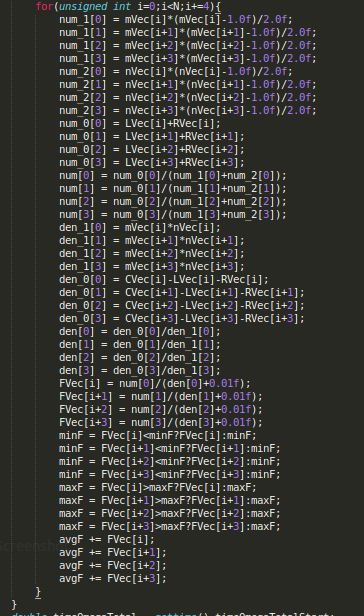
\includegraphics[scale=0.8]{/home/zisk/Desktop/LAB41839849/photo/3.png}
  \null \vfill
  
  \vfill \null
\end{multicols}

\vspace{70mm}
\selectlanguage{english}
\subsubsection{Loop Unroll}


\selectlanguage{greek}
Παραθέτεται τμήμα της υλοποίησης\\
\begin{multicols}{2}
Οι νέες μεταβλητές έχουν μετατραπεί σε πίνακες με 4 \selectlanguage{english}floats. \selectlanguage{greek}Η ροή του προγράμματος είναι παρόμοια με το σειριακό κώδικα για την εκτέλεση των υπολογισμών
μέσω των νέων δεικτών. Εξαιτίας των εξαρτήσεων μεταξύ των πράξεων, η διαδικασία δεν επιδιώκει βελτίωση. Ο αριθμός των επαναλήψεων λιγοστεύει με όμοια αντιστοιχία με την οποία αντιπροσωπεύουν οι καταχωρητές στις νέες μεταβλητές. Δεν βελτιώνεται η ταχύτητα. Υπάρχει εκμετάλλευση των καταχωρητών του επεξεργαστή. Σε ακραίες περιπτώσεις όπου στις μεταβλητές υπάρχει μεγάλος αριθμός από καταχωρητές, ο επεξεργαστής μπορεί να είναι ανίκανος να προσφέρει του απαιτούμενους πόρους.
  \null \vfill

  \vfill \null

\columnbreak
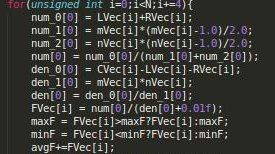
\includegraphics[scale=0.8]{/home/zisk/Desktop/LAB41839849/photo/1.jpg}
  \null \vfill
  
  \vfill \null
\end{multicols}

\vspace{20mm}
\subsubsection{Τελική Έκδοση \selectlanguage{english}SSE }
\selectlanguage{greek}\hspace*{8mm}Η έκδοση του \selectlanguage{english}SSE\selectlanguage{greek} έχει προκύψει ως ανάλυση των παραπάνω στοιχείων. Κάθε τετράδα \selectlanguage{english} \selectlanguage{greek}εντολών μετατρέπεται σε μια εντολή \selectlanguage{english} \selectlanguage{greek}όπως παρουσιάζεται στην εικόνα. Απαιτούνται καινούριες μεταβλητές \selectlanguage{english}vector \selectlanguage{greek}όπου η κάθε μία περιέχει μια τετράδα \selectlanguage{english}floats. \selectlanguage{greek}Η εντολές για την εκτέλεση των πράξεων ακολούθουν και αυτές \selectlanguage{english}vectorized \selectlanguage{greek}πρότυπα. \selectlanguage{greek}Οι εντολές λοιπόν, εκτελούνται παράλληλα και αυξάνεται το \selectlanguage{english} performance \selectlanguage{greek}του προγράμματος. Ορισμένα ενδιάμεσα βήματα των υπολογισμών ( προσθεσεις,αφαιρέσεις στον αριθμητη/παρανομαστη) τοποθετούνται ως παράμετροι στις συναρτήσεις. Έτσι το πρόγραμμα χρησιμοποιεί λιγότερους πόρους στους υπολογισμούς, και αυτό αποτυπώνεται στην περαιτέρω βελτίωση του χρόνου. \\


 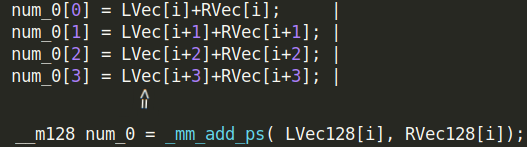
\includegraphics[scale=0.8]{/home/zisk/Desktop/LAB41839849/photo/5.png}
\vspace{15mm}
\subsubsection{\selectlanguage{english}SSE $\&$\  Pthreads }

\selectlanguage{greek}\hspace*{8mm}Η υλοποιήση με την χρήση \selectlanguage{english}Pthreads \selectlanguage{greek} απαιτεί ως επιπρόσθετη είσοδο τον αριθμό των \selectlanguage{english}threads. \selectlanguage{greek} Αναγκαία είναι η κατασκευή δυο \selectlanguage{english}struct \selectlanguage{greek}με τις απαραίτητες πληροφορίες για κάθε \selectlanguage{english}thread. \selectlanguage{greek}\\Στο πρώτο \selectlanguage{english}struct \selectlanguage{greek} εμπεριέχονται οι μεταβλητές
\begin{itemize}
\selectlanguage{greek}
\item Ταυτότητα του \selectlanguage{english} thread (ID) \selectlanguage{greek}
\item Συνολικός αριθμός \selectlanguage{english}threads
\item Executed Operation
\item Barrier
\item \selectlanguage{english}Index \selectlanguage{greek} των υπολογισμών που διαχειρίζονται
\end{itemize} 
\hspace*{8mm}Στο δεύτερο \selectlanguage{english}struct \selectlanguage{greek} εμπεριέχονται οι δείκτες του \selectlanguage{english}SSE\selectlanguage{greek} μοντέλου που χρησιμοποιούνται στους υπολογισμούς, αλλά και οι μεταβλητές για τα \selectlanguage{english} avg,min,max. \selectlanguage{greek}Εμπεριέχεται ως στοιχείο της πρώτης δομής.

Αρχικά το \selectlanguage{english} master thread \selectlanguage{greek} κανονίζει τη δέσμευση μνήμης για τους πίνακες που θα χρησιμοποιηθούν για τους υπολογισμούς. Οι πίνακες αυτοί θα αποτελέσουν στοιχείο του κάθε \selectlanguage{english} thread. \selectlanguage{greek}Γίνεται το \selectlanguage{english}initialization \selectlanguage{greek}των μεταβλητών μέσα σε μία \selectlanguage{english}for() \selectlanguage{greek}όπου το \selectlanguage{english}master thread \selectlanguage{greek} δημιουργεί τα απαιτούμενα (τόσα όσα είναι και ο αριθμός των \selectlanguage{english} thread) structs\selectlanguage{greek}. Τα νέα νήματα στέλνονται με την \selectlanguage{english} pthread$\_$create()  \selectlanguage{greek}στη συνάρτηση \selectlanguage{english} threadFUNC \selectlanguage{greek}  που γίνονται οι υπολογισμοί. Έπειτα τα \selectlanguage{english} threads \selectlanguage{greek} βρίσκονται σε κατάσταση \selectlanguage{english} busywait \selectlanguage{greek}και αναμένουν τα υπόλοιπα \selectlanguage{english}thread ($barrier=1$).\selectlanguage{greek} Ο \selectlanguage{english}master \selectlanguage{greek}πριν ξεκινήσει πρέπει να έχει δημιουργήσει και να στείλει τα υπόλοιπα, οπότε δεν υπάρχει νόημα να δημιουργηθεί το \selectlanguage{english}struct \selectlanguage{greek}του πρώτο. Για αυτόν τον λόγο η \selectlanguage{english}for() \selectlanguage{greek}είναι ανάποδη, δηλαδή ξεκινάει απο το τελευταίο νήμα και τελειώνει με το πρώτο. H ανάποδη υλοποίηση αποδείχτηκε ελαφρά πιο γρήγορη και επιλέχτηκε . Μέσα στα \selectlanguage{english} iterations, \selectlanguage{greek} υπολογίζονται τα \selectlanguage{english} indexes \selectlanguage{greek} που θα διαχειριστούν τα \selectlanguage{english} threads \selectlanguage{greek} στους υπολογισμούς. Σύμφωνα με τα \selectlanguage{english} indexes \selectlanguage{greek}αυτά, τα \selectlanguage{english}threads \selectlanguage{greek} σε κάθε \selectlanguage{english}iteration \selectlanguage{greek}θα διαχειριστούν διαφορετικά κομμάτια από τους πίνακες που βρίσκονται στο \selectlanguage{english} data struct  \selectlanguage{greek} και συνεπώς επιτυγχάνεται καλή διαχείριση τους. Πραγματοποιούνται οι υπολογισμοί  απο τα \selectlanguage{english} worker threads \selectlanguage{greek} σύμφωνα με το μοντέλο \selectlanguage{english} SSE\selectlanguage{greek} που έχει χρησιμοποιηθεί. Μετα το πέρας του υπολογισμού τους αναμένουν τον συγχρονισμό τους. Οι ζητούμενες μεταβλητές \selectlanguage{english} max,min,avg \selectlanguage{greek} υπολογίζονται ανατρέχοντας για κάθε \selectlanguage{english} thread \selectlanguage{greek}, την εκάστοτε παράμετρο και ελέγχοντας την με τις αντίστοιχες τιμές των υπολοίπων \selectlanguage{english} thread. \selectlanguage{greek}Για το \selectlanguage{english} average \selectlanguage{greek} γίνεται πρόσθεση των τιμών. Αν υπάρχει υπόλοιπο στην κατάτμηση της εισόδου στα \selectlanguage{english} threads \selectlanguage{greek} τότε ο υπολοιπόμενος υπολογισμός πραγματοποιείται από το \selectlanguage{english} master thread.\selectlanguage{greek} Στο τέλος της συνάρτησης τα  \selectlanguage{english} threads \selectlanguage{greek} σκοτώνονται. Χρονομετρείται ολόκληρη η διαδικασία.


\vspace{20mm}
\subsection{\selectlanguage{english}SSE $\&$\  Pthreads $\&$\ MPI }
\selectlanguage{greek}\hspace*{8mm}Το \selectlanguage{english} MPI \selectlanguage{greek} παρέχει παραλληλισμό σε επίπεδο πράξεων. Μεταχειρίζεται το φόρτο στις διεργασίες. Στο περιβάλλον αυτό, αρχικά πραγματοποιούνται οι απαραίτητες αρχικοποιήσεις ώστε να επικοινωνούν οι διεργασίες. Σε \selectlanguage{english} MPI\selectlanguage{greek} προγράμματα, χρησιμοποιείται η εντολή \selectlanguage{english} MPI$\_$Init(). \selectlanguage{greek}Η συνάρτηση αυτή επιτρέπει την επικοινωνία μεταξύ των \selectlanguage{english}processes \selectlanguage{greek}και είναι η πρώτη συνάρτηση που εκτελείται\selectlanguage{greek}. Κάθε διεργασία γνωρίζει το σύνολο των υπόλοιπων διεργασιών αλλα και την προτεραιότητα τους. Αυτό πραγματοποιείται με τις εντολές \selectlanguage{english} MPI$\_$Comm$\_$size \& MPI$\_$Comm$\_$rank \selectlanguage{greek}αντίστοιχα. Να σημειωθεί ότι στο \selectlanguage{english} struct \selectlanguage{greek} των \selectlanguage{english} thread\selectlanguage{greek} έχει συμπεριληφθεί η ταυτότητα της διεργασίας. Πλεον η κάθε διεργασία έχει τα δικά της \selectlanguage{english} threads \selectlanguage{greek} και οι υπολογισμοί γίνονται παράλληλα. Ο αριθμός των \selectlanguage{english}iterations \selectlanguage{greek} έχει ελαττωθεί στη μονάδα. Τα \selectlanguage{english} threads \selectlanguage{greek} εκτελούν τους υπολογισμούς κάθε διεργασίας. Η μεθοδολογία που χρησιμοποιείται για  τους υπολογισμούς μεσω \selectlanguage{english} thread \selectlanguage{greek} δεν έχει υποστεί διαφοροποίηση. 

Ορίζονται οι τύποι μεταβλητών με χρήση \selectlanguage{english}MPI$\_$FLOAT$\_$INT \selectlanguage{greek}και το περιβάλλον των διεργασιών με χρήση \selectlanguage{english}MPI$\_$COMM$\_$WORLD. \selectlanguage{greek}Η αποστολή των μυνημάτων γίνεται μια φορά πρίν την εκτύπωση του μέγιστου ώστε η επικοινωνία και η ανταλλαγή δεδομένων να είναι η ελάχιστη δυνατή. Πραγματοποιείται με την εντολή \selectlanguage{english}MPI$\_$GATHER\selectlanguage{greek} ώστε η κύρια διεργασία να επιτελέσει τις συγκρίσεις μεταξύ των αποτελεσμάτων των υπολοίπων διεργασιών καθώς και των δικών της. Τέλος η συνάρτηση \selectlanguage{english}MPI$\_$Finalize() \selectlanguage{greek}καλείται με σκοπό να καταστρέψει το περιβάλλον επικοινωνίας των διεργασιών. Δεν εγγυάται το τερματισμό τους παρα μόνο την συνέχεια της κύριας διεργασιας. 

\subsection{\selectlanguage{english} Bonus }
\selectlanguage{greek}\hspace*{8mm}Σε αυτό το σημείο παρουσιάζεται η εναλλακτική υλοποίηση με εκμετάλλευση διαφορετικού \selectlanguage{english}memory layout \selectlanguage{greek}. Ο κώδικας για τις \selectlanguage{english}SSE \selectlanguage{greek}εντολές έχει δεχθεί τροποποιήσεις. Διαπιστώθηκε ότι ο κώδικας θα μπορουσε να τροποποιηθεί εκτελώντας την μέθοδο του \selectlanguage{english}jam\selectlanguage{greek} ,που όπως διαπιστώθηκε από τον αρχικό κώδικα, προκαλεί βελτίωση της απόδοσης. Δεν υπάρχουν εξαρτήσεις με τους επόμενους υπολογισμούς οπότε η προτεινόμενη μέθοδος είναι εφικτή. Οι \selectlanguage{english}vectorized\selectlanguage{greek} μεταβλητές έχουν τροποποιηθεί σε \selectlanguage{english}vectorized arrays \selectlanguage{greek} 4 θέσεων. Τα δεδομένα εισόδου διαχωρίζονται σε πιο μικρά κομμάτια(αυτή τη φορά $\frac{Ν}{16}$) και σε κάθε \selectlanguage{english} iteration \selectlanguage{greek} οι δείκτες επεξεργάζονται διαφορετικό κομμάτι δεδομένων( ο πρώτος δείκτης τα πρώτα  $\frac{Ν}{16}$ , ο δεύτερος τα επόμενα κλπ). Οι ίδιες εντολές ομαδοποιούνται. Επομένως οι πίνακες πλέον διαχειρίζονται διαφορετικα κομμάτια υπολογισμών. Οι παράμετροι \selectlanguage{english} avg,min,max \selectlanguage{greek} υπολογίζονται με όμοιο τρόπο μόνο.

\vspace{20mm}
\section{Αποτελέσματα}
\hspace*{8mm}Έχουν πραγματοποιηθεί οι απαραίτητοι υπολογισμοί που αποδίδουν στην έκφραση του \selectlanguage{english}performance \selectlanguage{greek}για τις διάφορες υλοποίησεις. Οι υπολογισμοί αυτοί αποτυπώνονται στα γραφήματα. Τα γραφήματα εστιάζουν στη διάρκεια των υπολογισμών καθώς και στη βελτίωση σε σχέση με την αρχική υλοποίηση. Η κάθε υλοποίηση δέχεται ως είσοδο τον ίδιο αριθμό δεδομένων Ν=10000000. Θεωρείται το πρώτο γράφημα, το γράφημα της χρονικής διάρκεια της κάθε υλοποίησης ενώ το δεύτερο διάγραμμα της έκθεσης του \selectlanguage{english}Speedup.\selectlanguage{greek}

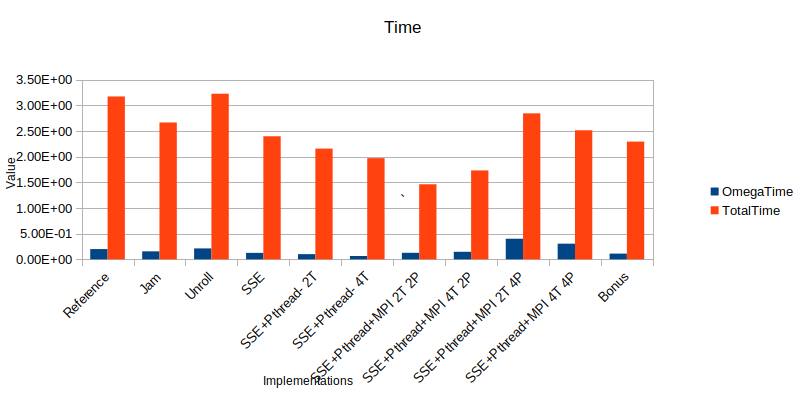
\includegraphics[scale=0.7]{/home/zisk/Desktop/LAB41839849/photo/Time.png}
\null \vfill
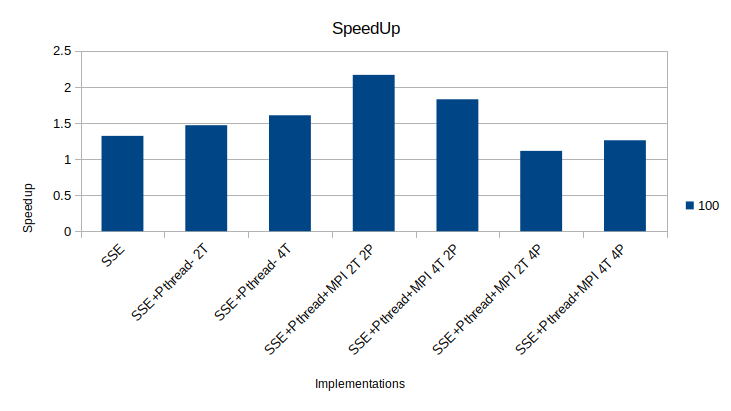
\includegraphics[scale=0.7]{/home/zisk/Desktop/LAB41839849/photo/SpeedUp.png}
\null \vfill
Επιπλέον, παρουσιάζεται ο πίνακας των αποτελεσμάτων από τα οποία εξήχθησαν τα παραπάνω γραφήματα.
\selectlanguage{english}
\begin{table}[h]
\begin{tabular}{ |p{3.5cm}||p{2cm}|p{2cm}| }
 \hline
 \multicolumn{3}{|c|}{\textbf{N = 10.000.000}} \\
 \hline
                     & Omega time	  & Total Time\\
 \hline
 Reference Code(RC)	& 0.19963s	    & 3.174151s\\
 RC with Loop Unroll    & 0.21263s        & 3.227579s\\
 RC with Jamming	    & 0.155849s        & 2.668166s\\
 SSE					& 0.126033s 			& 2.398806s\\
 SSE + 2 threads		& 0.101284s			& 2.158511s\\
 SSE + 4 threads		& 0.06446s			& 1.973034s\\
 SSE + 2 threads 2 procs		& 0.127441s		& 1.46363s\\
 SSE + 2 threads 4 procs		& 0.400856s		& 2.845927s\\
 SSE + 4 threads 2 procs		& 0.146648s		& 1.734404s\\
 SSE + 4 threads 4 procs		& 0.305505s		& 2.515387s\\
 Bonus						& 0.112597		& 2.295190s\\
  \hline
\end{tabular}
\end{table}

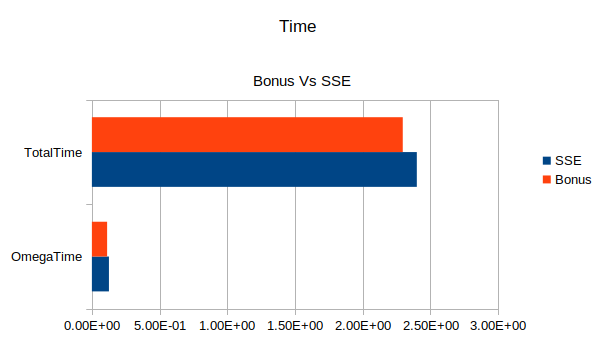
\includegraphics[scale=0.7]{/home/zisk/Desktop/LAB41839849/photo/bonustime.png}
\null \vfill
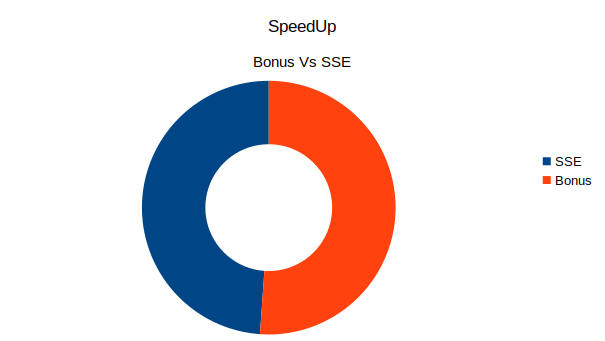
\includegraphics[scale=0.7]{/home/zisk/Desktop/LAB41839849/photo/bonusspeedup.png}
\null \vfill

\selectlanguage{greek}
\vspace{30mm}
Σύμφωνα με τα συμπεράσματα που εξάγονται από τα γραφήματα , σημειώνονται τα εξής:
\begin{enumerate}
\item Παρουσιάζεται βελτίωση από υλοποίηση σε υλοποίηση αναφορικά με την πρωτότυπη για κάθε τύπο παραλληλοποίησης.
\item Η χρήση καταχωρητών με το μοντέλο \selectlanguage{english}SSE \selectlanguage{greek}είναι αποδοτικό, καθώς οι μεταβλητές είναι ανεξάρτητες, οπότε δίνει μια εύκολη λύση για την επιτάχυνση του προγράμματος.
\item Ο συνδιασμός των δυο μεθόδων παραλληλοποίησης \selectlanguage{english}(SSE \& Pthread)\selectlanguage{greek} είναι σαφώς καλύτερος από την παραλληλοποίηση με \selectlanguage{english}SSE intrinsics\selectlanguage{greek}. Η βελτίωση μεγαλωνει με την αύξηση του αριθμού των \selectlanguage{english} threads. \selectlanguage{greek}Ο φόρτος ελαττώνεται με την αύξηση τους και υπάρχει καλύτερη εκμετάλλευση της παραλληλοποίησης.
\item Ο συνδιασμός των υλοποιήσεων δεν αποδίδει στη μέγιστη βελτίωση όπως διαισθητικά θα έπρεπε. Για μικρό αριθμό διεργασιών ανεξάρτητα του αριθμού των νημάτων, υπάρχει άριστη βελτίωση. Για αύξηση του αριθμού των διεργασιών, αυξάνεται το κόστος \selectlanguage{english}overhead \selectlanguage{greek} η δέσμευση πόρων , καθώς και η επικοινωνία μεταξύ τους. Αυτό αποδίδεται στους χρόνους εκτέλεσης και στην απόδοση.
\item Η προεραιτική υλοποίηση παρουσιάζει ελαφριά βελτίωση σε σχέση με την απλή υλοποίηση με εντολές \selectlanguage{english} SSE, \selectlanguage{greek} λόγω καλύτερης εκμετάλλευσης των καταχωρητών καθώς και των εξαρτήσεων που παρουσιάζουν οι εντολές μεταξύ τους.
\end{enumerate} 

\selectlanguage{greek}
Ως γενικό συμπέρασμα, το \selectlanguage{english}speedup \selectlanguage{greek} του \selectlanguage{english}SSE\selectlanguage{greek} επηρεάζεται από την φύση των υπολογισμών. Προσθέτωντας νήματα στην υλοποίηση, η απόδοση επηρεάζεται με την υπερβολική εκμετάλλευση των πόρων και την σωστή κατανομή του φόρτου σε αυτά. Αντίθετα στο\selectlanguage{english} MPI\selectlanguage{greek} είναι ανεξάρτητο από τις πράξεις, όμως επηρεάζεται από το μέγεθος των δεδομένων, την ανάγκη επικοινωνίας και τους πόρους που του διαθέτονται.

\vspace{15mm}
\selectlanguage{greek}
\section{Συμπεράσματα \& Παρατηρήσεις}
\hspace{8mm}Το \selectlanguage{english}SSE \selectlanguage{greek}αποτελεί αξιόπιστο και αποδοτικό πρότυπο παραλληλοποίησης για ορθή και δομημένη υλοποίηση. Προσφέρει πληθόρα εντολών η οποία επεκτείνεται στους νέους επεξεργαστές. \selectlanguage{greek}Λόγω του ακριβή και εκτεταμένου \selectlanguage{english}documentation, \selectlanguage{greek}το \selectlanguage{english}API \selectlanguage{greek}αποδίδει τα αναμενόμενα αποτελέσματα. Μειονέκτημά του είναι η αδυναμία εκτέλεσης αποδοτικών πράξεων μεταξύ των στοιχείων ενός \selectlanguage{english}vector,\selectlanguage{greek} κάτι που αποφεύγεται ή μειώνεται με καλύτερη δόμη στον κώδικα. Τέλος το \selectlanguage{english}speedup \selectlanguage{greek}έχει ανώτατο όριο πόσα δεδομένα χωράνε ταυτόχρονα στο \selectlanguage{english}pipeline\selectlanguage{greek} του επεξεργαστή. 

Το \selectlanguage{english}MPI \selectlanguage{greek}προσφέρει μείωση του χρόνου λειτουργίας.Εξαρτάται όμως από πολλούς παράγοντες όπως αναφέρθηκε στα αποτελέσματα των\selectlanguage{english} speedups. \selectlanguage{greek}Με τη βοήθεια λογισμικού όπως το \selectlanguage{english}LAM, \selectlanguage{greek}το\selectlanguage{english} MPI \selectlanguage{greek}έχει προοπτικές για βελτίωση του\selectlanguage{english}speedup,\selectlanguage{greek} γιατί ενδέχεται να συγχρονίσει παραπάνω από έναν υπολογιστή και να δημιουργήσει ένα \selectlanguage{english}cluster \selectlanguage{greek}επεξεργαστών. Υπάρχουν έτοιμες συναρτήσεις όπως η \selectlanguage{english}MPI$\_$GATHER$()$ \selectlanguage{greek}που προσφέρουν μεγαλύτερη ταχύτητα και  βελτιωμένη λειτουργικότητα. Τέλος ένα μειωνέκτημα του είναι η αβεβαιότητα για το πως επιδρούν ορισμένες συναρτήσεις στον κώδικα. Λόγου χάρη, δε γίνεται να είναι γνωστό ακριβώς ποιες διεργασίες συνεχίζουν μετά το \selectlanguage{english}MPI$\_$Finalize$()$.\selectlanguage{greek}

 Τα\selectlanguage{english} Pthreads \selectlanguage{greek}δεν έχουν αυτοματοποιημένη λειτουργικότητα. Χρονοβόρα στη δημιουργία της υλοποίησης και στο συγχρονισμό με ευθύνη του δημιουργού την διασφαλίση της επικοινωνίας μεταξύ των \selectlanguage{english}thread \selectlanguage{greek}. Τα οφέλη τους είναι η δυνατότητα αλλαγής και βελτίωσης χαρακτηριστικών, καθώς και γνώση της ακριβούς λειτουργικότητας του κώδικα. 
 
 Η παραλληλοποίηση μέσω των \selectlanguage{english}Pthreads \selectlanguage{greek}με εντολές\selectlanguage{english} SSE \selectlanguage{greek}είναι αισθητή και αναμενόμενη στη βελτίωση του \selectlanguage{english} speedup. \selectlanguage{greek}Αντίθετα ο συνδιασμός \selectlanguage{english}SSE , Pthreads \& MPI\selectlanguage{greek} καθώς διευσθητικά βελτίωνει ακομά περισσότερο σε σχέση με \selectlanguage{english}SSE \& Pthread  \selectlanguage{greek} η βελτίωση δεν είναι η αναμενόμενη. Η περαιτέρω δέσμευση των πόρων είναι αυτή που εμποδίζει αυτην την βελτίωση.
 
 Η διαισθητική προσέγγιση για την απόδοση της παραλληλοποίηση μέσω των \selectlanguage{english}Pthreads \& MPI \& SSE \selectlanguage{greek} θα μπορουσε να εκφραστεί ως πολλαπλή βελτίωση καθώς η μεμονομένη υλοποίηση τους βελτιώνει την αρχική υλοποίηση. Θεματα συγχρονισμού και \selectlanguage{english} overhead \selectlanguage{greek} αποφέρουν χειρότερα αποτελέσματα στην απόδοση τελικά. Στην κατάσταση της απόδοσης να προστεθεί βέβαια και το μέγεθος των δεδομενων (στη συγκεκριμένη περίπτωση είναι μεγάλος όγκος όπου χειροτερεύει το \selectlanguage{english} communication)

\selectlanguage{greek}Εν κατακλείδι, το \selectlanguage{english}SSE, \selectlanguage{greek}και γενικά τα \selectlanguage{english}SIMD \selectlanguage{greek}πρότυπα, είναι ανεξάρτητα από το μεγέθος των δεδομένων, όμως θέτεται ανώτατο όριο στο \selectlanguage{english}speedup \selectlanguage{greek}από τον επεξεργαστή και το πάχος του \selectlanguage{english}pipeline \selectlanguage{greek}. Αντίθετα, το \selectlanguage{english}MPI \selectlanguage{greek}αντιμετωπίζει δυσκολίες ανάλογα τον όγκο δεδομένων αλλά έχει υψηλό \selectlanguage{english}scalability.\selectlanguage{greek} Το ανώτατο φράγμα του \selectlanguage{english}speedup \selectlanguage{greek} ορίζεται από τους πόρους που του διαθέτονται.

\end{document}
